% Chapter Template

\chapter{Ensayos y resultados} % Main chapter title
En este capitulo se explica las pruebas realizadas al hardware, firmware , controladores y a la plataforma IoT a lo largo del trabajo.
\label{Chapter4} % Change X to a consecutive number; for referencing this chapter elsewhere, use \ref{ChapterX}

%----------------------------------------------------------------------------------------
%	SECTION 1
%----------------------------------------------------------------------------------------

\section{Pruebas Unitarias}
Para el desarrollo de los drivers del modulo BG96 y el sensor AHT10 se utilizo la metodologia de desarrollo TDD.Esto implica que se escribieron pruebas unitarias para los drivers.
Una forma cuantitativa de evaluar estas pruebas son los informes de cobertura generados por ceedling,la herramienta utilizada para ejecutar las pruebas automaticas.

En la figura \ref{fig:Cobertura aht10} se puede observar el informe de cobertura del driver aht10, donde se puede apreciar que las pruebas ejecutan el 100\% de las lineas de codigo escritas y explora el 100\% de las conbinaciones en los saltos de condicionales.

En la figura \ref{fig:Cobertura BG96} tambien se observa el informe de cobertura del dirver de BG96, con 98.4\% de lineas ejecutadas y explora mas del 98.3\% de combinaciones posibles. 

\begin{figure}[h!]
    \centering
      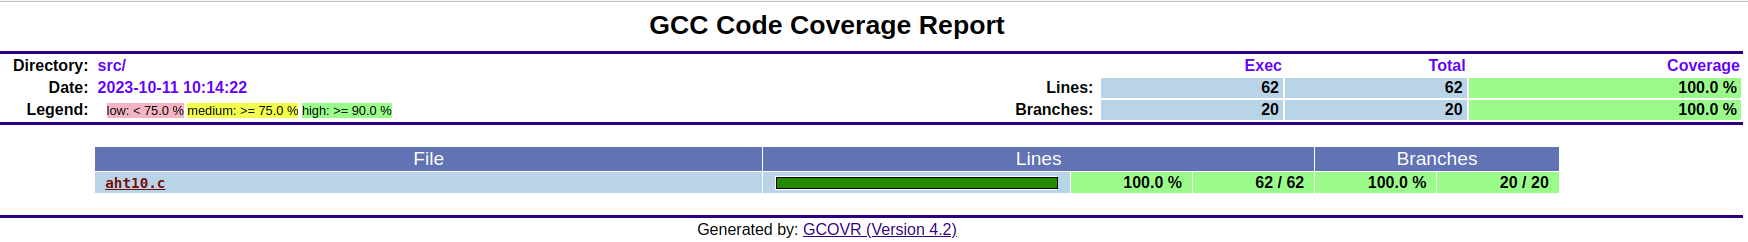
\includegraphics[width=\linewidth, height=6cm]{./Figures/cobertura_aht10.png}
    \caption{Informe de cobertura driver aht10.}
      \label{fig:Cobertura aht10}
  \end{figure}

\begin{figure}[htbp!]
    \centering
      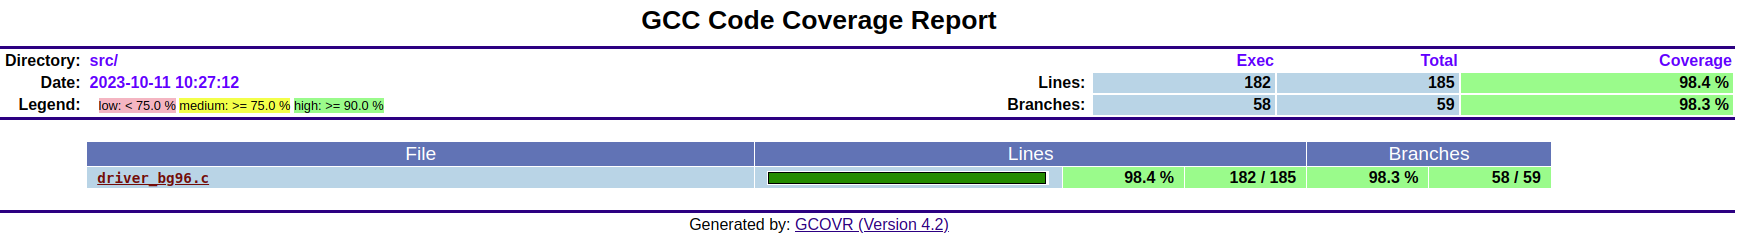
\includegraphics[width=\linewidth, height=6cm]{./Figures/cobertura_bg96.png}
    \caption{Informe de cobertura driver BG96.}
      \label{fig:Cobertura BG96}
\end{figure}
  

\vspace{4cm} 
\section{Pruebas De Hardware}
\subsection{Prueba sensor de humedad AHT10}
Para probar el correcto funcionamiento del sensor AHT10 y la correcta comunicacion con el microcontrolador se comprobo la trama I2C con un analizador logico,
en la figura podemos ver la trama capturada donde observamos como el sensor 

\subsection{Pruebas sensor analogicos}
Prueba sensor de humedad de suelo

Pruebas de aalimetaccion del modulorealzado

\subsection{Pruebas comunicacion por UART con modulo de comunicacion}

Para probar la comunicacion del microcontrolador con el modulo por UART se utlizo un abnalizador logico que nos permite los comandos que envia el microcontrolador y la respuestas del modulo a estos comandos.
En la figura podemos ver esta comunicacion bidirecional por puerto AURT.
\subsection{Pruebas bajo consumo }
Al se un dispositivo que funcionara a bateria lo que busca el firmware consumir lo menos posible, lo que se hizo fue hacer hacer la lectura de los sensores y enviar los datos cada 15min y el el tiempo restante mandar el microcontrolador a bajo consumo 
En la figura podemos ver el consumo del sistema normalmente y eb bajo consumo.



\section{Pruebas del firmware}
\subsection{Pruebas de conexion con broker mqtt}
Una de las tareas mas importante del firmware es la del manejo del servidor,para verficar el correcto funcionamiento de esta tarea tenemos que ver la secuencia de comandos que son mandados del microcontroaldor al modulo de comunicion por el puerto UART.

En la figura podemos observar toda la secuencia de envio de datos a la plataforma Iot, primeramente el modulo optine un apn del proveedor del red, luego



\subsection{Pruebas de alarmas}
El objetivo de esta prueba es comprobar el buen funcionamiento de las alarmas del sistema.
Cuando la humedad del suelo baja por debajo del rango permitido por el sistema, el firmware manda un sms al usuario con la alarma ocurrida.En la figura podemos ver que la humedad bajo de 5\% y en la figura se resibio el sms.




\section{Pruebas de la plataforma IoT}
\subsection{Pruebas de inyeccion de mensajes}
El objetivo de las pruebas de la plataforma IoT es evaluar la llegada de los mensajes por protocolo MQTT.
Para su realizacion se utilizo la aplicación de linea de comandos de mosquitto.
Para realizar el envio de datos a broker MQTT, se utiliza el cliente MQTT de mosquitto utilizando el comando que se muestra en la figura .


Donde:

Posterior a ejecutar el comando podemos ver lo que se es es conectar el servidor , enviar 

Para comprobar la llegada de los valores al broker de ThingsBoard tenemos que ir a la seccion dispositivos, seleccionar el dispositivo al que se le envio los datos y entrar a la pestana de ultima telemetria, en la figura podemos ver que los datos llegaron correctamente.





\label{sec:pruebasHW}

